\section{Game objects management}
A game object, such as a humanoid-looking bot or a car most often can be understood as existing in three different planes simultaneously:
\begin{enumerate}
    \item the visual layer,
    \item the physical layer,
    \item the logical layer.
\end{enumerate}
The visual layer of an object describes how the object looks like during the gameplay.
This side of a game object we will call a \textit{model}.
The information about models (vertices, normal vectors, UV mappings, textures, and animations) is read from COLLADA and PNG files (see \autoref{subsec:model_loader-class}) and stored in the \texttt{Model} class.
It's important to note that if multiple game objects look the same, the model information is shared between them in the form of a single \texttt{ModelResource} class instance.
More specifically, the \texttt{ModelResource} class is abstract, and its derived classes are singletons.
Animated models additionally use the \texttt{Aminator} class (see \autoref{subsec:animator-class}) which provides a way to calculate the bone transforms based on the elapsed time.
Some models are \textit{compound}.
The car model, for example, stores information about the look of the wheels and body separately.

The physical layer defines the physical properties of the game object at any given moment.
Some basic ones include inertia, angular and linear velocity, and friction;
in the case of more complex objects such as a car, the description contains information about \textit{constraints}.
The constraints define the relative positions of different elements of the object and their velocities.
An example of a constraint would be the wheel axes of the car.
It's worth noting that the position constraints don't have to be "stiff" (they are modeled as springs).
Technically, once a game object is added to the simulation, it is represented by one (or more in the case of compound bodies) \textit{body handle}.
Therefore, each game object has to implement the \texttt{ISimulationMember} interface which has a property that returns the list of all body handles associated with the given game object.
More details on coupling the physics engine with the rest of the game can be found in \autoref{subsec:physics-project}

The logical layer is the soul of each object.
NPCs move in a way given by a simple algorithm;
the player can inflict damage to NPCs by shooting projectiles, and so on.
Game objects can react to collisions with other objects by registering for contact callbacks, i.e. implementing the \texttt{IContactEventListener} interface.
They can also move (either on their own, like NPCs, or due to the player input) by registering input callbacks, i.e. implementing the \texttt{IInputSubscriber} interface (see \autoref{subsec:context-class} and \autoref{subsec:transporter-classes}).
The logic related to game objects of a given kind is usually contained in a respective Controller class, described in more detail in \autoref{subsec:controller-classes}.

All game objects are members of a scene (see \autoref{subsec:scene-class}).

In the remainder of this section, we will cover some of the most important components related to managing game objects.
\subsection{\texttt{Animator} class}\label{subsec:animator-class}

The \texttt{Animator} class is responsible for animating the models loaded by \texttt{ModelLoader}.
It takes animation keyframes and interpolates them using Quaternion Slerp and Vector3 Lerp which are provided by AssimpNet.
It then uses the interpolated keyframes to calculate the transformation matrices for each bone in the model which are later passed to the shader.
The logic is described in more detail in \autoref{sec:theory_theory_models}.
\subsection{\texttt{ModelLoader} class}\label{subsec:model_loader-class}

The model loader is responsible for loading models from the file system.
It loads COLLADA files using AssipmNet to convert them to model class objects.
Each vertex in the mesh of the model must be dependent on at most 4 bones.
It creates VAOs for each mesh of the model, stores them in the Model class object, loads a PNG file, and stores it in a Texture class object.

\subsection{\texttt{Physics} project}\label{subsec:physics-project}
The Physics component is responsible for collision detection, ray casting, and physical modeling.
The main purpose of this component is to expose the various functionalities of the BepuPhysics2 library to the rest of the system.
The component also makes extensive use of the code from the BepuPhysics2 Demos project.

Each game object is represented by a \textit{body} (each body has an associated \textit{body handle}) in the physics engine.
This one-to-one mapping is stored in the \texttt{Scene} class in an object of \texttt{SimulationMembers} type.
\texttt{SimulationMembers} allows for adding and removing simulation members as well as accessing handles to bodies in the physics engine associated with a given game object.
Game objects are represented by either simple or composite shapes in the physical simulation.
Simple shapes used in the game include cylinders, capsules, and boxes.
Composite shapes arise by composing simple shapes.

To facilitate debugging, the Physics component also provides a way to extract all shapes from the simulation (and decompose composite shapes) which then can be shown in debug mode, see \autoref{fig:bounding-shapes}.
When shown, the bounding shapes can be either green or red depending on whether the corresponding bodies are in the active or inactive state in the physics engine.
In \autoref{fig:bounding-shapes} it can be seen that the player has been hit by a projectile which caused the player's body to become active (or \textit{awakend} using the BepuPhysics parlance) as indicated by the green bounding shape.
The projectile that hit the player can also be seen to be active.
On the other hand, the projectiles that fell to the ground and had been still for some time became inactive as marked by the red bounding shapes.
\begin{figure}[h]
    \centering
    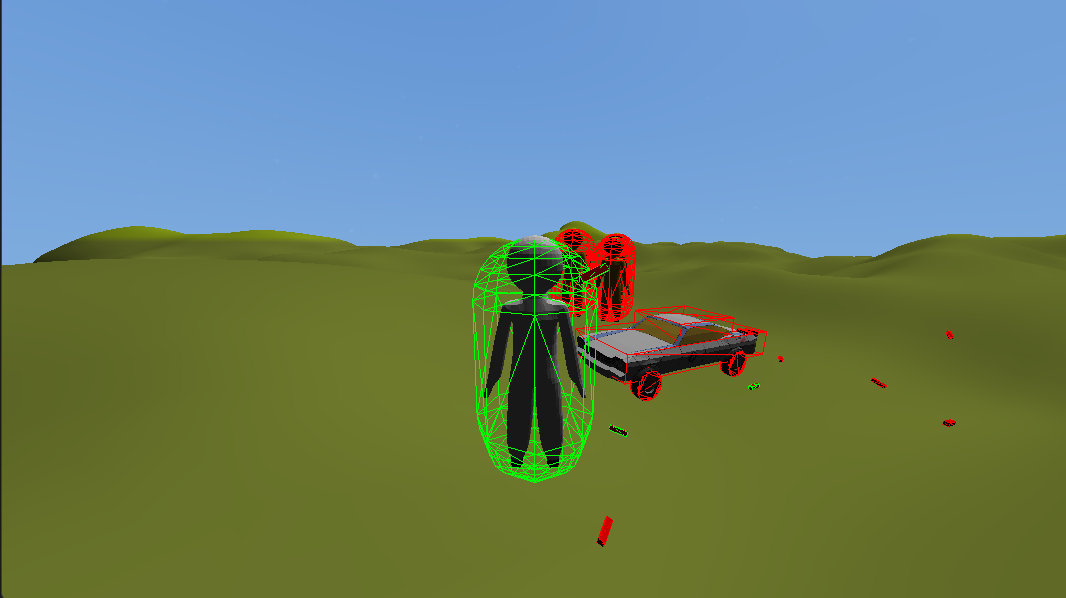
\includegraphics[width=0.8\textwidth]{chapters/implementation/sections/game_objects_management/subsections/physics_project/resources/bounding-shapes.png}
    \caption{Game objects enclosed in bounding shapes for collision detection}
    \label{fig:bounding-shapes}
\end{figure}

The body that represents the terrain was created as a separate shape from the terrain mesh triangle-by-triangle.

Game objects can listen and respond to collisions by registering their contact callbacks via the API in \texttt{SimulationManager}.
Such objects implement the \texttt{IContactEventListener} interface whose implementations define the contact callbacks.
The only information about the collision is which two bodies collided and where.

Some game objects can cast rays.
An example of such an object is the player who uses a ray to define a place where terrain modification should take place.
Each ray in the physics engine has an ID number, direction, etc.
An object that wishes to cast rays has to therefore implement an interface (\texttt{IRayCaster}) that exposes all the necessary information.
\subsection{\texttt{Scene} class} \label{subsec:scene-class}
The \texttt{Scene} class is responsible for storing all the objects in the game the player can interact with.
It is also responsible for releasing the objects' resources.
Some of the objects stored in the \texttt{Scene}'s instance are the following: car, chunks, player, camera, etc.
\subsection{\texttt{*Controller} classes}
There are eight controller classes in the project:
\texttt{PlayerController},
\texttt{BotsController},
\texttt{ChunksController},
\texttt{ProjectilesController},
\texttt{VehiclesController},
\texttt{LightSourcesController},
\texttt{HudController},
\texttt{BoundingShapesController}, and
\texttt{SkyboxController}.

All the controller classes serve the same purpose.
They exist to render objects and deal with object callbacks.
For example, \texttt{ProjectilesController} renders all existing projectiles and also removes the dead projectiles from the scene.
Each projectile has a \texttt{IsAlive} property which is read every time a render frame callback is called by the controller to check if the projectile is still alive.

\subsection{\texttt{*Transporter} classes}
The Transporter component is vital for the spherical geometry mode of the game.
It is responsible for transporting game objects between spheres.
All transporters implement the \texttt{ITransporter} interface.

Each game object has a property \texttt{CurrentSphereId} that attains one of two values: 0 or 1 depending on which sphere the object is currently in (this property is a part of \texttt{ISimulationMember} interface).
Whenever an object moves, the Transporter determines whether it should be transported to the opposing sphere by calculating the object's distance from its current sphere's center.

The transportation process changes the object's position and velocity.
In the case of objects modeled as compound bodies, it is necessary to alter the positions and velocities of each of the components.
When a camera is attached to an object that gets transported, it also has to be updated accordingly.
More specifically, the Transporter transforms the camera's front vector and updates the information about the camera's current sphere.

The functionalities mentioned above are only relevant in the spherical geometry mode.
To make the system design consistent across all modes, there is also a \texttt{NullTransporter} implementation of the \texttt{ITransporter} interface which is used in hyperbolic and Euclidean geometry modes.
This is a dummy class with methods that don't do anything.
\subsection{\texttt{Context} class}
The Context component is responsible for input handling and performing actions on each frame.
There are two sources of user input considered in the video game: keyboard and mouse.
Keys and mouse buttons can be in one of three states: \textit{pressed}, \textit{down}, and \textit{up}.
Additionally, the mouse can also generate events when it's moved.

The \texttt{Context} class stores mappings between different types of input and actions that should be triggered by the given input.
Changes in the input state are tracked by OpenTK and the \texttt{Context} activates relevant actions as a response.
It is a convention that every class that registers new actions in the \texttt{Context} implements the \texttt{IInputSubscriber} interface.
Also, it is worth noting that, for better performance, the Context will only trigger actions associated with the input that has itself been previously registered.